% Shared float (common/make_floats.py). Figure: figures/generative_ablations.pdf
\begin{figure}[htbp]
\centering
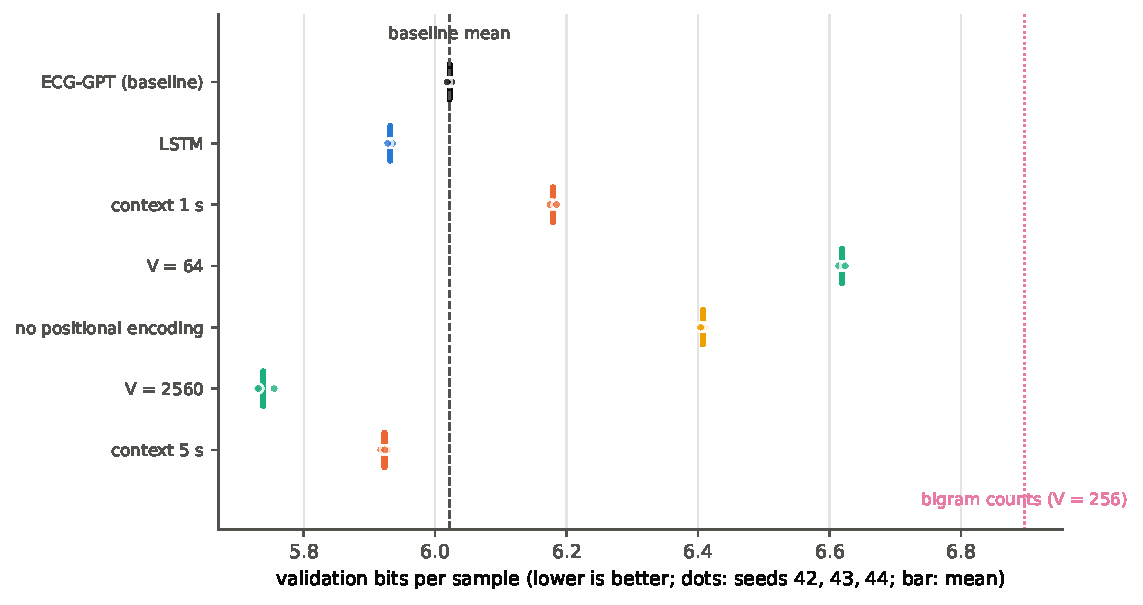
\includegraphics[width=\textwidth,height=0.42\textheight,keepaspectratio]{figures/generative_ablations.pdf}
\caption[Generators: ablations in bits per sample]{Generator ablations: validation bits per sample (lower is better; dots: seeds 42, 43, 44; bar: mean; dashed line: baseline mean; dotted: bigram counting model with $V = 256$).}
\label{fig:generative_ablations}
\end{figure}
